\documentclass{beamer}
\usepackage{luatexja}
\usepackage{graphicx}
\renewcommand{\kanjifamilydefault}{\gtdefault}
\usetheme{metropolis}
\title{DCONでのケージ案１}
\author{MEKOU}
\date{\today}

\begin{document}
\begin{frame}
    \titlepage
\end{frame}

\begin{frame}
    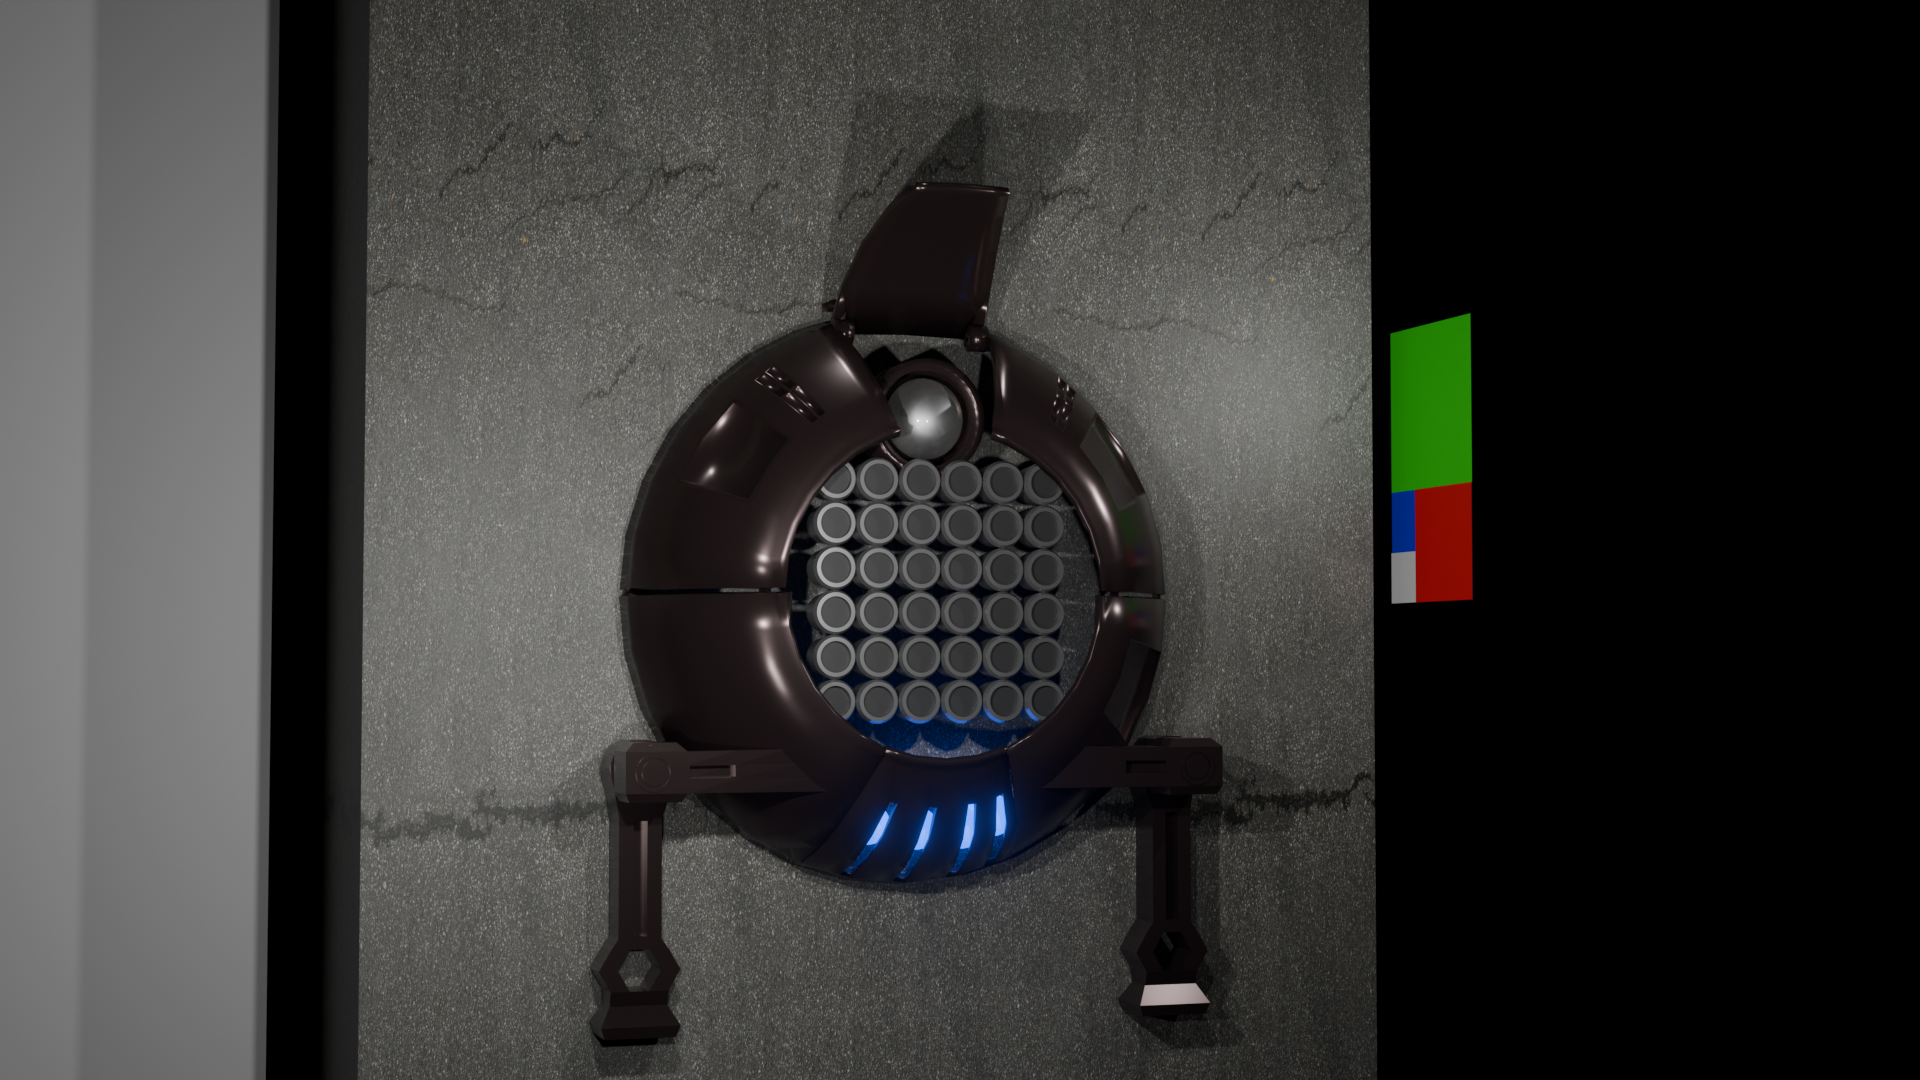
\includegraphics[width=0.4\textwidth]{./render1.png}
    実際に埋め込まれたパターン
    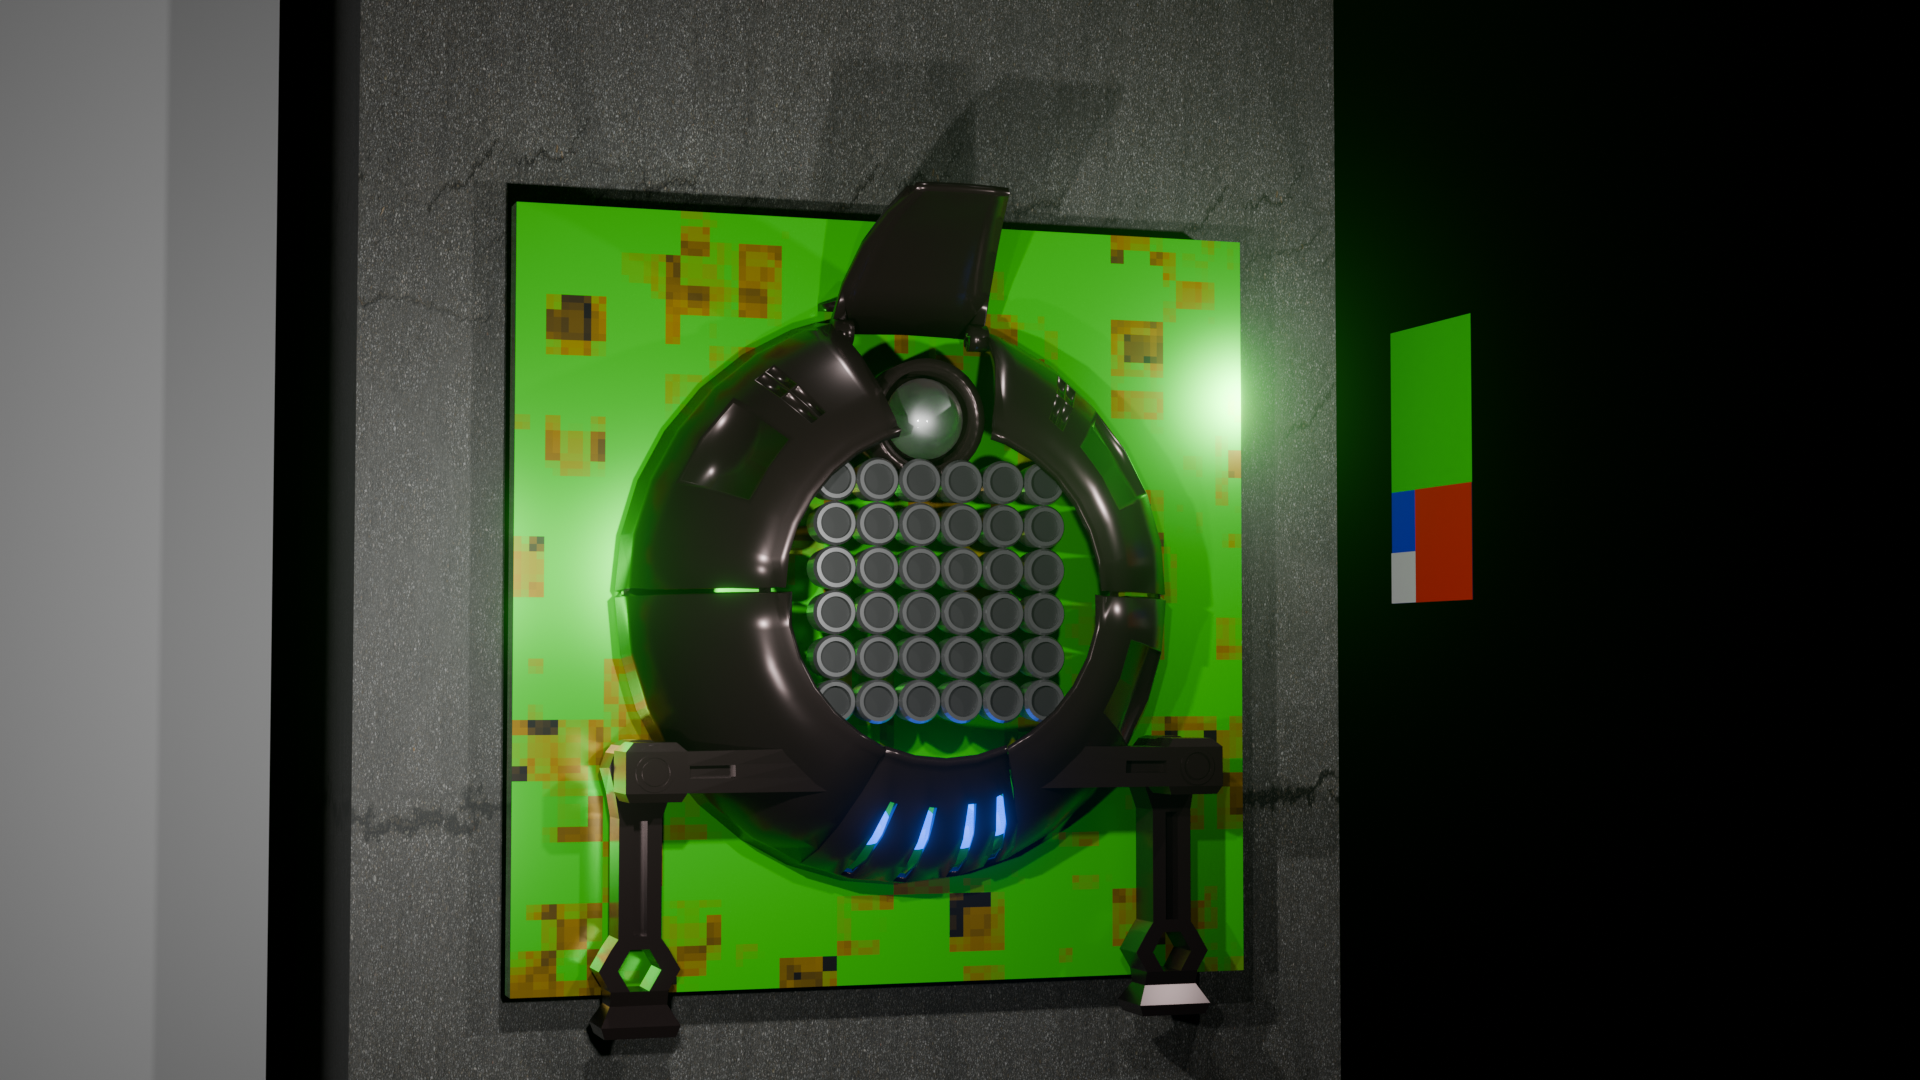
\includegraphics[width=0.4\textwidth]{./render2.png}
    基盤との接続部分のイメージ
    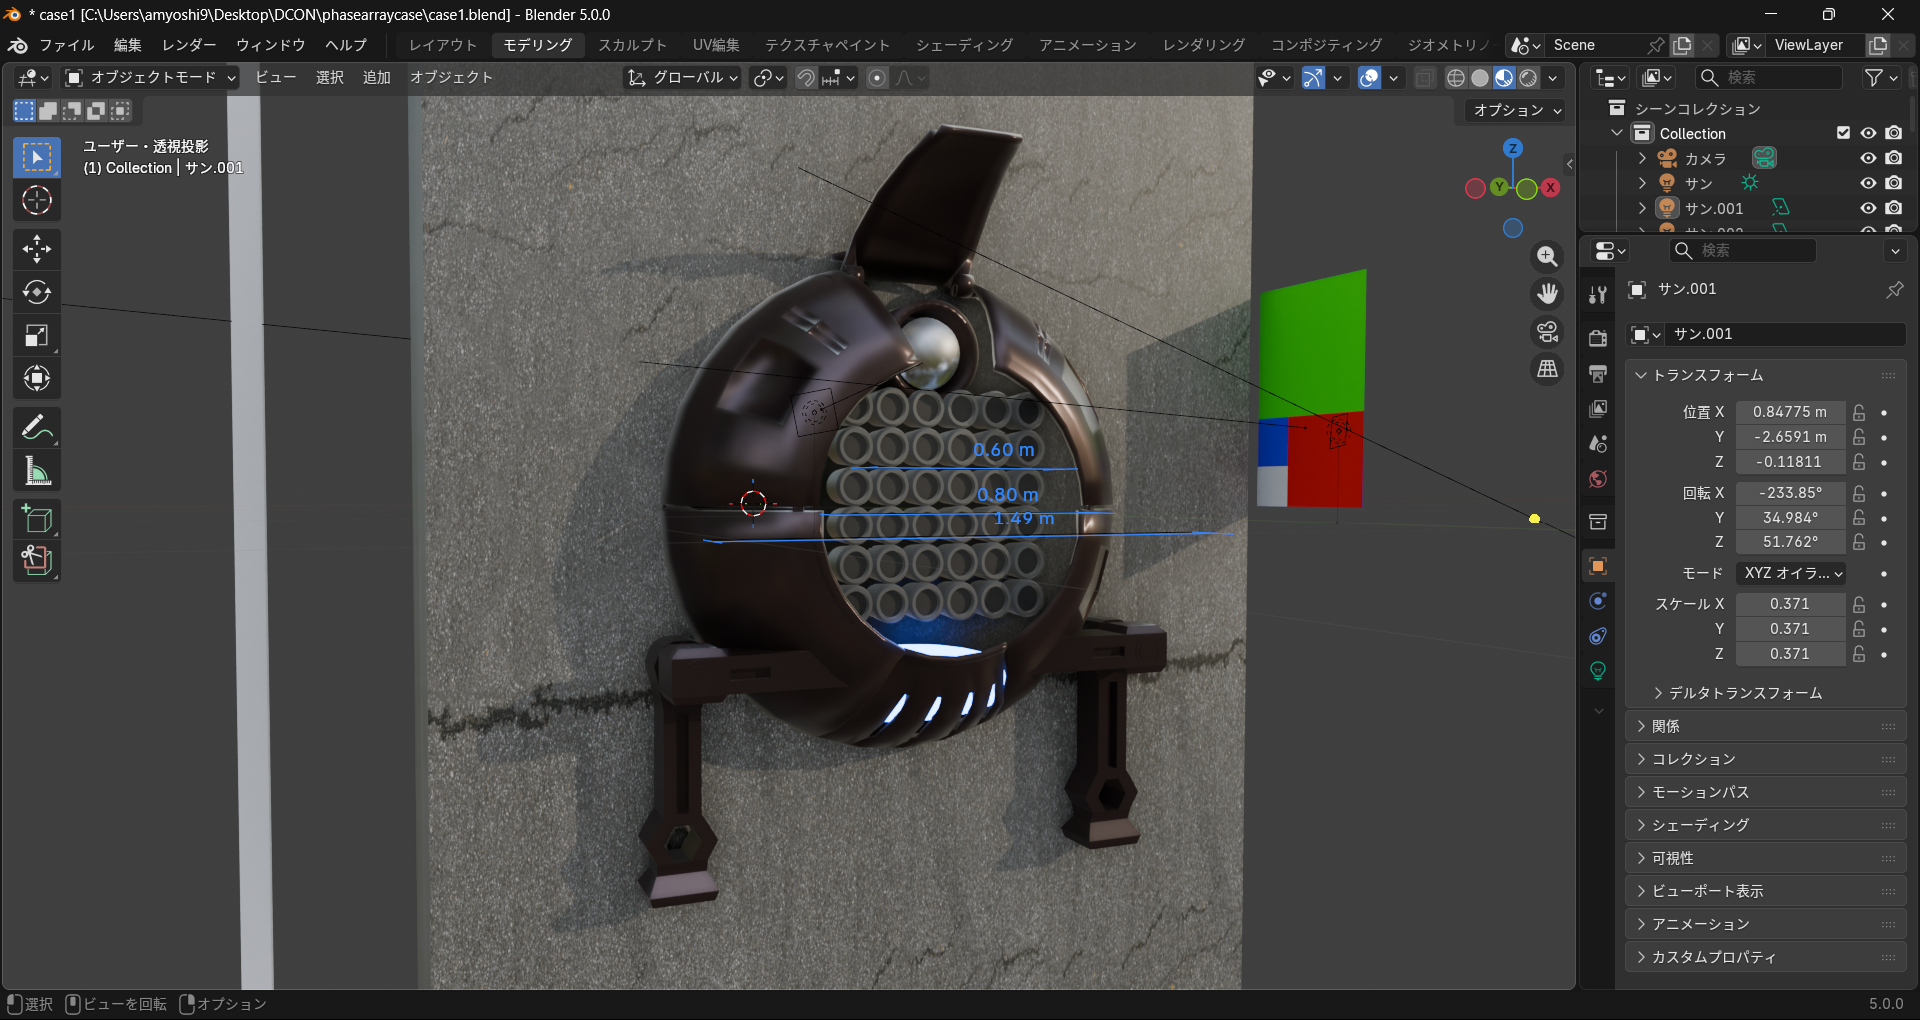
\includegraphics[width=0.4\textwidth]{./render3.png}
    レンダーがきれいだったバージョン

    
    下部の足が稼働できるので、柱などと固定ができる
\end{frame}


\end{document}